\documentclass[12pt]{article}
\usepackage[left=1cm, right=1cm, top=2cm,bottom=1.5cm]{geometry} 

\usepackage[parfill]{parskip}
\usepackage[utf8]{inputenc}
\usepackage[T2A]{fontenc}
\usepackage[russian]{babel}
\usepackage{enumitem}
\usepackage[normalem]{ulem}
\usepackage{amsfonts, amsmath, amsthm, amssymb, mathtools}

\usepackage{fancyhdr}
\pagestyle{fancy}
\renewcommand{\headrulewidth}{1.5pt}
\renewcommand{\footrulewidth}{1pt}

\usepackage{graphicx}
\usepackage[figurename=Рис.]{caption}
\usepackage{subcaption}
\usepackage{float}

%%Наименование папки откуда забирать изображения
\graphicspath{ {./images/} }

%%Изменение формата для ввода доказательства
\renewcommand{\proofname}{$\square$  \nopunct}
\renewcommand\qedsymbol{$\blacksquare$}

\addto\captionsrussian{%
	\renewcommand{\proofname}{$\square$ \nopunct}%
}
%% Римские цифры
\newcommand{\RN}[1]{%
	\textup{\uppercase\expandafter{\romannumeral#1}}%
}


\theoremstyle{definition}
\newtheorem{defn}{Опр:}
\newtheorem{rem}{Rm:}
\newtheorem{prop}{Утв.}
\newtheorem{exrc}{Упр.}
\newtheorem{lemma}{Лемма}
\newtheorem{theorem}{Теорема}
\newtheorem{corollary}{Следствие}

\newenvironment{cusdefn}[1]
{\renewcommand\thedefn{#1}\defn}
{\enddefn}



\DeclareRobustCommand{\divby}{%
	\mathrel{\text{\vbox{\baselineskip.65ex\lineskiplimit0pt\hbox{.}\hbox{.}\hbox{.}}}}%
}
\DeclareMathSymbol{\shortminus}{\mathbin}{AMSa}{"39}

\newcommand{\smallerrel}[1]{\mathrel{\mathpalette\smallerrelaux{#1}}}
\newcommand{\smallerrelaux}[2]{\raisebox{.1ex}{\scalebox{.75}{$#1#2$}}}

\newcommand{\smallin}{\smallerrel{\in}}
\newcommand{\smallnotin}{\smallerrel{\notin}}

\newcommand*{\medcap}{\mathbin{\scalebox{1.25}{\ensuremath{\cap}}}}%
\newcommand*{\medcup}{\mathbin{\scalebox{1.25}{\ensuremath{\cup}}}}%

\begin{document}
	\lhead{Математический анализ - I}
	\chead{Шапошников С.В.}
	\rhead{Лекция - 15}

\section*{Предел функции и его свойства}

Говорят, что при $x \to a$ предел $f(x) = b$ или $\lim\limits_{x \to a}f(x) =b$, если $f\colon D \to \mathbb{R}$, $a$ - предельная точка $D$, $\forall \{x_n\} \in D, \, x_n \to a, \, x\neq a, \, f(x_n) \to b$.


\begin{defn}\textbf{(Коши)} 
	Пусть $f\colon D \to \mathbb{R}$, $a$ - предельная точка $D$. Число $b$ называется \uwave{пределом} $f$ при $x \to a$, если 
	$$\forall \varepsilon > 0, \, \exists \, \delta > 0 \colon \forall x \in D, \, 0 < |x-a| < \delta \Rightarrow |f(x) -b| < \varepsilon$$	
\end{defn}

\begin{figure}[H]
	\centering
	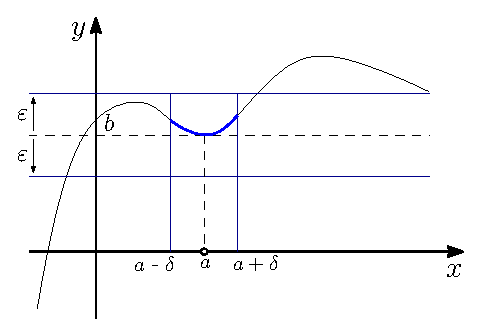
\includegraphics[width=0.45\textwidth]{15_1.eps}
	\caption{Определение предела функции $f(x)$.}
	\label{15_1}
\end{figure}

\begin{rem}
	$|x-a| > 0$ - то же самое, что и сказать $x \neq a$.
\end{rem}

\begin{rem}
	Если $D$ - не ограничено сверху, то в качестве $a$ можно взять $+\infty$ и \uline{определение Коши} переписывается так:
	$$\forall \varepsilon > 0, \, \exists \, M > 0 \colon \forall x \in D, \, x > M \Rightarrow |f(x) -b| < \varepsilon$$	
\end{rem}

 
\begin{rem}
	Если $D$ - не ограничено снизу, то в качестве $a$ можно взять $-\infty$ и \uline{определение Коши} переписывается так:
	$$\forall \varepsilon > 0, \, \exists \, M > 0 \colon \forall x \in D, \, x < -M \Rightarrow |f(x) -b| < \varepsilon$$	
\end{rem}

\begin{theorem}
	Определения Гейне и Коши - равносильны.
\end{theorem}

\begin{proof}Рассмотрим случай, когда $a$ - число. На бесконечности - аналогично\\
	(K) $\Rightarrow$ (Г): $\forall \varepsilon > 0, \, \exists \, \delta > 0 \colon \forall x \in D, \, 0 < |x-a| < \delta \Rightarrow |f(x) -b| < \varepsilon$. Пусть $x_n \in D, \, x_n \to a$ и $x_n \neq a$. По определению предела последовательности $\exists \, N \colon \forall n > N, \, 0 < |x_n - a| < \delta \Rightarrow |f(x_n) - b | < \varepsilon \Rightarrow f(x_n) \to b$ и выполняется определение Гейне.
	
	(Г) $\Rightarrow$ (К): $\forall \{x_n\} \in D, \, x_n \to a \wedge x_n \neq a$ верно, что $f(x_n) \to b$. Предположим, что определение Коши не выполняется $\Rightarrow \exists \, \varepsilon > 0, \, \forall \delta > 0, \, \exists \, x \in D \colon 0 < |x - a| < \delta \wedge |f(x) - b| \geq \varepsilon$. Пусть $\delta = \dfrac{1}{n}$, тогда найдется $x_n \colon 0 < |x_n - a| < \dfrac{1}{n} \wedge |f(x_n) - b| \geq \varepsilon$. Тогда $x_n \to a \wedge x_n \neq a$, но $|f(x_n) - b| \geq \varepsilon$, то есть $f(x_n) \nrightarrow b \Rightarrow$ противоречие.
\end{proof}

\begin{theorem} \textbf{(Ограниченность)}:
	Пусть $x \in D, \, \lim\limits_{x \to a} f(x) = b$. Тогда $\exists \, \mathcal{U}^\prime(a) \wedge C > 0 \colon |f(x)| \leq C, \, \forall x \in \mathcal{U}^\prime(a) \cap D$. Если у функции в точке есть предел, то в некоторой проколотой окрестности эта функция должна быть ограничена.
\end{theorem}

\begin{proof}
	Используем определение Коши, пусть $\varepsilon = 1 \Rightarrow \exists \, \delta > 0  \colon \forall x \in D, \, \underbrace{0 < |x - a| < \delta}_{x \smallin \mathcal{U}_\delta^\prime(a)} \Rightarrow |f(x) - b| < 1$. Тогда получим следующее:
	$$\forall x \in \mathcal{U}_\delta^\prime(a) \cap D, \, |f(x)| \leq |f(x) - b| + |b| < 1 + |b| = C$$
\end{proof}

\begin{exrc}
	Доказать с помощью определения Гейне.
\end{exrc}

\begin{theorem} \textbf{(Отделимость)}:
	Пусть $x \in D, \, \lim\limits_{x \to a} f(x) = b > 0 \Rightarrow \exists \, \mathcal{U}^\prime(a) \colon \forall x \in \mathcal{U}^\prime(a) \cap D, \, f(x) \geq \dfrac{b}{2} > 0$.
\end{theorem}

\begin{proof}
\begin{figure}[H]
	\centering
	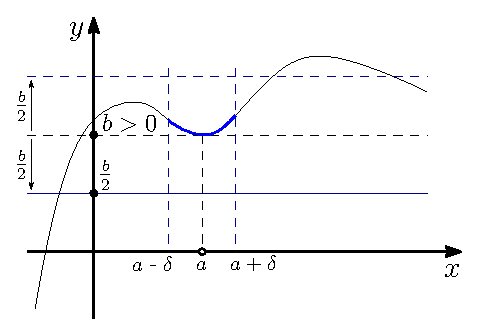
\includegraphics[width=0.45\textwidth]{15_2.eps}
	\caption{Доказательство теоремы отделимости.}
	\label{15_2}
\end{figure}
Возьмем $\varepsilon =\dfrac{b}{2}, \, \exists \, \delta > 0 \colon \forall x \in D, \, 0 < |x - a| < \delta \Rightarrow |f(x) - b| < \dfrac{b}{2}$. Тогда 
$$\forall x \in \mathcal{U}_{\delta}^\prime(a) \cap D, \, f(x) = f(x) - b + b \geq -\dfrac{b}{2} + b = \dfrac{b}{2}$$ 
\end{proof}

\begin{exrc}
	Доказать с помощью определения Гейне.
\end{exrc}

\newpage

\section*{Замечательные пределы}

\subsection*{$(\RN{1})$ Первый замечательный предел} 

$$\lim\limits_{x \to 0} \dfrac{\sin{x}}{x} = 1$$

\begin{rem}
	Множество $D = \mathbb{R} \setminus 0$. Но будем рассматривать только $x \in (-\frac{\pi}{2}, \frac{\pi}{2}) \setminus \{0\}$, так как нас интересует поведение функции около $0$.
	
	Заметим также, что $\dfrac{\sin{x}}{x}$ - четная функция, поэтому будем рассматривать $0 < x < \dfrac{\pi}{2}$.
\end{rem}
\begin{proof}
	
Заметим, что $2 \sin{x} \leq 2x$, то есть хорда не длиннее дуги. Тогда $\sin{x} \leq x \Rightarrow \dfrac{\sin{x}}{x} \leq 1$.
\begin{figure}[H]
	\centering
	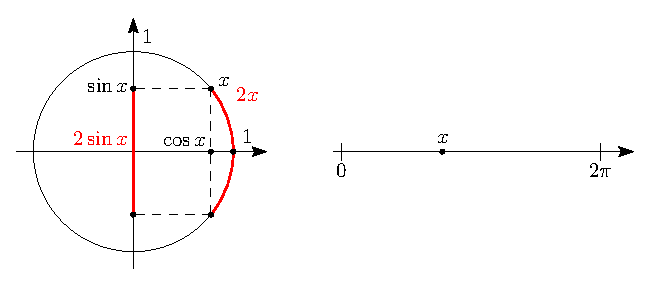
\includegraphics[width=0.65\textwidth]{15_3.eps}
	\caption{Хорда не длиннее дуги.}
	\label{15_3}
\end{figure}

Найдем $\tan{x}$ и обозначим вершины соответствующего сектора и треугольника:

\begin{figure}[H]
	\centering
	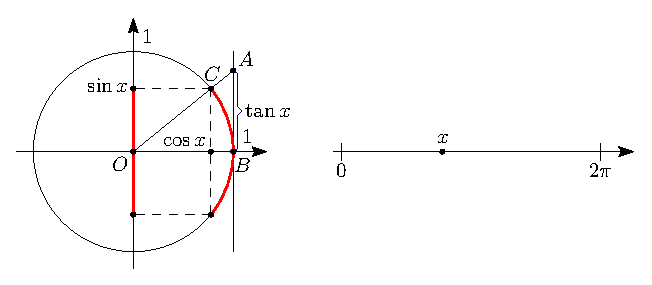
\includegraphics[width=0.65\textwidth]{15_4.eps}
	\caption{Треугольник $OAB$ содержит сектор $OCB$.}
	\label{15_4}
\end{figure}

Сектор $OCB \subset OAB \Rightarrow S_{OCB} \leq S_{OAB}$. Площадь сектора $=$ доля сектора от всего круга на площадь круга. Доля сектора $=$ доля дуги от длины всей окружности. Доля дуги $= \dfrac{x}{2\pi}$, площадь круга $= \pi r^2 = \pi\cdot 1^2 = \pi \Rightarrow S_{OCB} = \pi\cdot \dfrac{x}{2\pi} = \dfrac{x}{2} \leq S_{OAB} = \dfrac{\tan{x}}{2} \Rightarrow \cos{x} \leq \dfrac{\sin{x}}{x}$. 

Так как $|\sin{x}| \leq |x|$, то по теореме о двух полицейских $\lim\limits_{x\to 0} \sin{x} = 0$. $\lim\limits_{x \to 0}\cos{x} = \lim\limits_{x \to 0}\Big(1 - 2 \sin^2{\frac{x}{2}}\Big) = 1$.

По теореме о двух полицейских, из того, что $\cos{x} \leq \dfrac{\sin{x}}{x} \leq 1$ в интервале $(-\frac{\pi}{2}, \frac{\pi}{2}) \setminus \{0\}\Rightarrow$ 
$$\lim\limits_{x \to 0} \cos{x} = 1 = \lim\limits_{x \to 0} 1 \Rightarrow \lim\limits_{x \to 0}\dfrac{\sin{x}}{x} = 1$$
\end{proof}

\begin{rem}
	Важно заметить, что понятия площади круга, площади сектора, длины дуги в данном случае не определены строго и доказательство первого замечательного предела становится циклическим.
\end{rem}

\subsection*{$(\RN{2})$ Второй замечательный предел} 

$$\lim\limits_{x \to +\infty} \bigg(1 + \dfrac{1}{x}\bigg)^x = e$$

Знаем, что $\lim\limits_{n \to \infty}\big(1 + \frac{1}{n}\big)^n = e$. Используя это знание докажем второй замечательный предел.

\begin{proof}
	Пусть $n \leq x < n+1 \Rightarrow$ 
	$$\bigg(1 + \frac{1}{x}\bigg)^x \leq \bigg(1 + \frac{1}{n}\bigg)^x \leq \bigg(1 + \frac{1}{n}\bigg)^{n+1}$$
	$$\bigg(1 + \frac{1}{n+1}\bigg)^n \leq \bigg(1 + \frac{1}{n+1}\bigg)^x \leq \bigg(1 + \frac{1}{x}\bigg)^x$$
	
	Так как $\lim\limits_{n \to \infty}\big(1 + \frac{1}{n}\big)^{n+1} = \lim\limits_{n \to \infty}\big(1 + \frac{1}{n+1}\big)^n =e$, то 
	$$\forall \varepsilon >0, \, \exists \, N \colon \forall n > N, \, \bigg(1 + \frac{1}{n}\bigg)^{n+1} < e + \varepsilon \wedge \bigg(1 + \frac{1}{n+1}\bigg)^n > e - \varepsilon$$
	
	Пусть $x > N + 1$, тогда $x$ точно заключен между $n$ и $n+1 \colon n > N$. Получим
	
	$$e - \varepsilon < \bigg(1 + \frac{1}{n+1}\bigg)^n \leq \bigg(1 + \frac{1}{x}\bigg)^x \leq \bigg(1 + \frac{1}{n}\bigg)^{n+1} <  e + \varepsilon \Rightarrow$$
	$$\Rightarrow \bigg|\bigg(1 + \frac{1}{x}\bigg)^x - e\bigg| < \varepsilon$$
	
\end{proof}

\begin{exrc}Докажите, что:
	\begin{enumerate}[label={(\arabic*)}]
		\item $\lim\limits_{x \to -\infty}{(1 + \frac{1}{x})^x} = e$;
		\item $\lim\limits_{x \to 0}{(1 + x)^\frac{1}{x}} = e$;
	\end{enumerate}
\end{exrc}

Как узнать, есть ли у последовательности предел или нет? Аналогично пределам последовательности есть теорема Вейрштрасса и критерий Коши.

\begin{defn}
	Пусть $D^- = (-\infty, a) \cap D$, $D^+ = (a, +\infty) \cap D$. 
	
	Если $a$ - предельная точка $D^-$, то предел функции $f$ по множеству $D^-$, при $x \to a$ называется \uwave{пределом слева} и обозначается, через $\lim\limits_{x \to a\shortminus} f(x)$ или $\lim\limits_{x \to (a-0)}f(x)$ или $f(a-0)$.
	
	Если $a$ - предельная точка $D^+$, то предел функции $f$ по множеству $D^+$, при $x \to a$ называется \uwave{пределом справа} и обозначается, через $\lim\limits_{x \to a+} f(x)$ или $\lim\limits_{x \to (a+0)}f(x)$ или $f(a+0)$.
\end{defn}

\textbf{Распишем с точки зрения Гейне и Коши}: для $\lim\limits_{x \to a\shortminus}f(x)$

\uline{Гейне}: $\forall \{x_n\} \in D, \, x_n \to a \wedge x_n < a$ верно, что $f(x_n) \to b$.

\uline{Коши}: $\forall \varepsilon > 0,\, \exists \, \delta > 0 \colon \forall x \in D,\, a -\delta < x < a \Rightarrow |f(x) - b| <\varepsilon$.

\textbf{Пример}: Рассмотрим следующую функцию $f(x)$:
\begin{figure}[H]
	\centering
	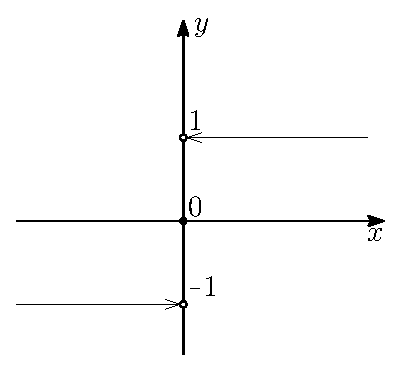
\includegraphics[width=0.30\textwidth]{15_5.eps}
	\caption{Пример разных частичных пределов слева и справа.}
	\label{15_5}
\end{figure}

Существуют пределы справа и слева: $\lim\limits_{x \to 0-}f(x) = -1$, $\lim\limits_{x \to 0+}f(x) = 1$, но в точке $0$ предела $\lim\limits_{x \to 0}f(x)$ не существует.

\begin{theorem}
	Пусть $a$ - предельная точка $D^-$ и $D^+$. Тогда $$\lim\limits_{x\to a}f(x) = b \Leftrightarrow \lim\limits_{x\to a\shortminus}f(x) = b \wedge \lim\limits_{x\to a+}f(x) = b$$
\end{theorem}
\begin{proof}\hfill\\
	$(\Rightarrow)$ По определению Коши $\forall \varepsilon > 0,\, \exists \, \delta > 0 \colon \forall x \in D,\, a -\delta < x < a + \delta \Rightarrow |f(x) - b| <\varepsilon$. Тогда\\ 
	$\forall x \in D,\, a -\delta < x < a \Rightarrow |f(x) - b| <\varepsilon \wedge \forall x \in D,\, a < x < a + \delta \Rightarrow |f(x) - b| <\varepsilon \Rightarrow$\\
	 $\Rightarrow \lim\limits_{x\to a\shortminus}f(x) = b \wedge \lim\limits_{x\to a+}f(x) = b$.
	
	$(\Leftarrow)$ По определению Коши $\forall \varepsilon > 0,\, \exists \, \delta_1 > 0 \colon \forall x \in D,\, a -\delta_1 < x < a \Rightarrow |f(x) - b| <\varepsilon$, \\
	 $\exists \, \delta_2 > 0\colon \forall x \in D,\, a < x < a + \delta_2 \Rightarrow |f(x) - b| <\varepsilon$. Пусть $\delta = \min\{\delta_1,\delta_2\}$, тогда как только \\
	 $a - \delta < x < a + \delta, \, x \neq a \Rightarrow |f(x) - b| < \varepsilon$.
\end{proof}

\begin{theorem}\textbf{(Вейрштрасса)}
	Пусть $f\colon D \to \mathbb{R}$ не убывает и ограничена сверху. Пусть $a$ - предельная точка $D^-$. Тогда существует $\lim\limits_{x \to a\shortminus}f(x) = \sup\limits_{x \in D^-} f(x)$.
\end{theorem}
\begin{rem}
	$D^- = (-\infty, a)$, тогда из $x \in D^- \Rightarrow x < a$.
\end{rem}
\begin{proof}
	\begin{figure}[H]
		\centering
		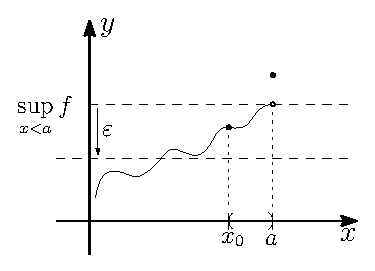
\includegraphics[width=0.35\textwidth]{15_6.eps}
		\caption{Доказательство теоремы Вейрштрасса.}
		\label{15_6}
	\end{figure}

	$\forall \varepsilon > 0$ число $\sup\limits_{D^-}f -\varepsilon$ не является верхней гранью значений $f$ на множестве $D^-$. Следовательно, $\exists \, x_0 \in D^- \colon f(x_0) > \sup\limits_{D^-}f - \varepsilon$. Из-за монотонности $f$, $\forall x \in (x_0, a) \cap D \Rightarrow f(x) \geq f(x_0) \Rightarrow$ 
	$$\sup\limits_{D^-}f - \varepsilon < f(x) \leq \sup\limits_{D^-}f, \, \forall x \in (x_0,a)\cap D$$
	
	Дельту можно взять, как $\delta = a - x_0$.
\end{proof}

\begin{rem}
	Аналогично доказываются следующие утверждения:
	\begin{figure}[H]
		\begin{subfigure}[b]{0.5\textwidth}
			\centering
			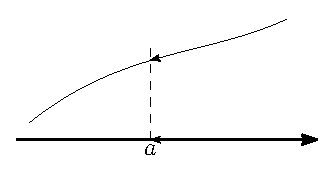
\includegraphics[width=0.5\textwidth]{15_7.eps}
			\caption{Не убывает и ограничена снизу.}
			\label{15_7}
		\end{subfigure}%
		\begin{subfigure}[b]{0.5\textwidth}
			\centering
			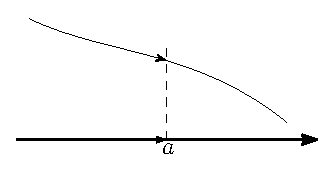
\includegraphics[width=0.5\textwidth]{15_8.eps}
			\caption{Не возрастает и ограничена снизу.}
			\label{15_8}
		\end{subfigure}
	\end{figure}
	\begin{enumerate}[label={\arabic*)}]
		\item Если $f$ не убывает на $D$, ограничена снизу и $a$ - предельная точка $D^+$, то $\lim\limits_{x \to a+}f = \inf\limits_{D^+}f$;
		\item Если $f$ не возрастает на $D$, ограничена снизу и $a$ - предельная точка $D^-$, то $\lim\limits_{x \to a\shortminus}f = \inf\limits_{D^-}f$;
		\item Если $f$ не возрастает на $D$, ограничена сверху и $a$ - предельная точка $D^+$, то $\lim\limits_{x \to a+}f = \sup\limits_{D^+}f$;
	\end{enumerate}
\end{rem}

\begin{corollary}
	Если $f$ - монотонная функция на интервале $(\alpha, \beta)$, то в каждой точке интервала существуют пределы $f$ слева и справа.
\end{corollary}

\begin{figure}[H]
	\centering
	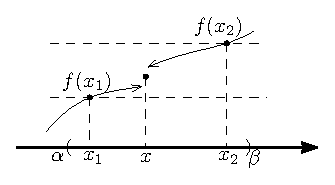
\includegraphics[width=0.3\textwidth]{15_9.eps}
	\caption{Следствие теоремы Вейрштрасса. }
	\label{15_9}
\end{figure}
$f(x_1)$ и $f(x_2)$ - ограничивают значения функции $f$ снизу и сверху. По теореме Вейрштрасса есть предел слева и справа.
\end{document}